\documentclass[11pt]{article}
\usepackage[a4paper,margin=24mm,top=21mm,bottom=22mm]{geometry}
\usepackage[T1]{fontenc}
\usepackage{lmodern,amsmath,booktabs,graphicx,xcolor,hyperref}
\definecolor{ink}{HTML}{203447}
\definecolor{teal}{HTML}{006B61}
\hypersetup{colorlinks=true,linkcolor=teal,urlcolor=teal,citecolor=teal,
 pdftitle={Initializing QAOA pattern search on nonclustered target keys},
 pdfauthor={Variational Quantum Algorithms project}}
\input{glyphtounicode}\pdfgentounicode=1
\newcommand{\StarterRows}{%
Halton & 86.1 & 97.2 & 13.60 & 98.5 & 28.2 \\
Random & 66.0 & 79.3 & 23.46 & 89.8 & 27.9 \\
Sobol & 50.0 & 68.1 & 29.90 & 84.9 & 28.6 \\
Original, joint & 43.1 & 66.7 & 32.78 & 82.8 & 30.2 \\
Recursive, joint & 43.1 & 66.7 & 32.53 & 82.8 & 30.2 \\
Original, coordinate & 65.3 & 73.6 & 24.47 & 85.2 & 26.8 \\
Recursive, coordinate & 65.3 & 73.6 & 24.50 & 85.5 & 26.9 \\
Immediate pattern search & 61.1 & 69.4 & 26.38 & 84.3 & 21.6 \\
}
\newcommand{\DecisionRows}{%
Immediate pattern search & 1.0 & 45 & 49 & 26.10 & 21.9 \\
Fixed 8 & 8.0 & 39 & 40 & 34.67 & 22.8 \\
Fixed 13 & 13.0 & 63 & 66 & 16.00 & 27.7 \\
Fixed 33 & 33.0 & 58 & 72 & 13.56 & 45.3 \\
Halton only & 65.0 & 58 & 72 & 13.56 & 65.0 \\
Four-call patience & 8.0 & 36 & 37 & 38.19 & 23.5 \\
Learned 8 or 13 & 9.9 & 56 & 57 & 22.50 & 25.1 \\
}

\setlength{\parindent}{0pt}
\setlength{\parskip}{5pt plus .6pt minus .4pt}
\setlength{\tabcolsep}{5pt}
\renewcommand{\arraystretch}{1.14}
\newcommand{\sect}[2]{\noindent{\sffamily\bfseries\large\color{ink}#1\hspace{.6em}#2}\par\smallskip}
\newcommand{\subt}[1]{\smallskip\noindent{\sffamily\bfseries\color{teal}#1}\par}
\newcommand{\figcaption}[2]{{\small\textbf{Figure #1.} #2\par}}
\newcommand{\tabcaption}[2]{{\small\textbf{Table #1.} #2\par}}
\newcommand{\E}{\mathbb{E}}
\usepackage{amssymb}
\pagestyle{myheadings}
\markboth{Hybrid angle search for MaxCut}{\footnotesize\textsf{HYBRID ANGLE SEARCH FOR MAXCUT}}
\begin{document}
\thispagestyle{plain}
{\sffamily\small\color{teal}\bfseries VARIATIONAL QUANTUM ALGORITHMS PROJECT}\par
\vspace{3pt}
{\sffamily\bfseries\fontsize{24}{27}\selectfont\color{ink}\raggedright Initializing QAOA pattern search on nonclustered target keys\par}
{\large A recursive sieve, a Halton start, and the cost of the handoff\par}
{\small Research draft prepared for Pauli Rikula \hfill 21 November 2026\par}
\vspace{3pt}\noindent{\color{teal}\rule{\linewidth}{1pt}}
\subt{Abstract}
Does a recursive sieve give pattern search a better start when valid keys cluster? This paper establishes the nonclustered baseline using the quantum approximate optimization algorithm (QAOA) for MaxCut. Every valid key was isolated in the sieve's integer order in all 72 confirmation graph/start cases. \textbf{By call 65, a recursive start hit 47 of 72 targets, a Halton start hit 66, and immediate pattern search hit 49.} Both hybrids used 13 starting calls and the same local search. In the companion experiment, putting those same valid energies into one solid block reversed the ranking, with 79.0\% hits for the recursive hybrid and 73.8\% for Halton \cite{clusterstudy}. This comparison uses a controlled reindexing of the energy table.

\sect{1}{Why spend 13 calls on initialization?}
The original study compared two sieves and pattern search on five MaxCut graphs with three starts each \cite{rikula,farhi}. On evaluation 13, the original sieve, recursive sieve and pattern search had reached 10, 9 and 8 targets. On evaluation 14 their counts were 10, 9 and 13. This crossing motivated our split. We spend 13 calls sampling and start local polling from the best sampled point on call 14. We also compare 33-call starts and adaptive switches. A cluster means consecutive valid keys in the sieve's integer encoding. The fact that two pairs of angles are physically close is a different condition.

\begin{center}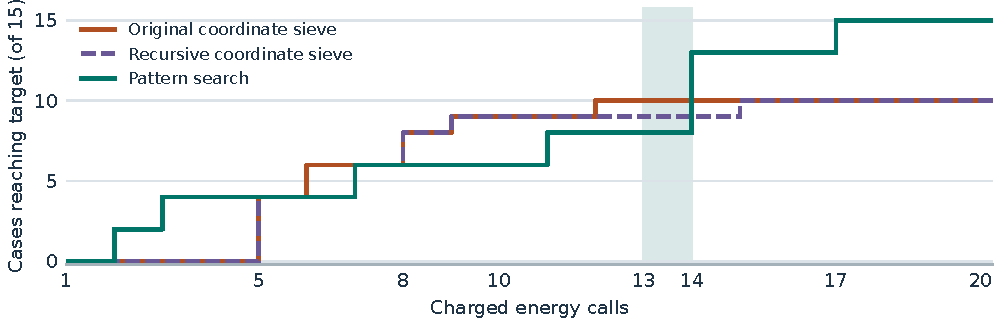
\includegraphics[width=.92\linewidth]{figures/crossover.pdf}\end{center}
\figcaption{1}{Historical cumulative target hits at each paid evaluation. The shaded interval marks the change from call 13 to 14. These curves start each algorithm from the common initial point. A hybrid instead starts its local phase at the best sampled point, which changes the comparison.}

\newpage
\sect{2}{A common optimizer and a common budget}
On an $M\times M$ periodic grid, $M=2^b$, each point $(g,h)$ indexes the angles $(2\pi g/M,2\pi h/M)$. Set $H_C|z\rangle=-\mathrm{cut}(z)|z\rangle$. The exact noiseless state and minimized energy are
\[
  |\psi\rangle=e^{-i\beta\sum_jX_j}e^{-i\gamma H_C}|+\rangle^{\otimes n},
  \qquad E(\gamma,\beta)=\langle\psi|H_C|\psi\rangle.
\]
All methods pay for the same initial point and keep the earliest incumbent within a tolerance of $10^{-12}$. With cap $B$ and pilot fraction $f$, the pilot uses at most $k=\max(1,\lfloor fB+1/2\rfloor)$ calls. A single local search starts at its best evaluated point, so the handoff costs zero additional evaluations.

\tabcaption{1}{Seven pilot schedules. The five joint schedules translate their offsets by the common initial point, modulo $M$. The two coordinate controls preserve the order in the historical implementation.}
{\small\begin{tabular}{@{}p{.265\linewidth}p{.675\linewidth}@{}}\toprule
Pilot & Order of evaluated points\\\midrule
Original / recursive joint & Run the existing sieve on $2b$ bits. Split alternate key bits between the two angles, with the most significant bit assigned to $\gamma$ (Morton decoding). The two sieves differ within dyadic levels.\\
Halton / Sobol & Use unscrambled 2-D Halton (bases 2 and 3) or Sobol points. Floor each coordinate onto the grid. Skip repeated pilot cells and the initial cell before requesting energies \cite{halton,sobol}.\\
Random joint & Draw grid cells uniformly without replacement. Use the same 12 deterministic seeds for paired policy comparisons.\\
Original / recursive coordinate & Scan the absolute $\gamma$ grid, then $\beta$, fixing the other angle at each scan's start. Charge repeated queries to match the original study.\\\bottomrule
\end{tabular}}

Local polling fixes its center for a batch, tries $+\gamma,-\gamma,+\beta,-\beta$ at step $\pi/2$, repeats a successful step and halves an unsuccessful one. It stops below one grid spacing or at the budget. Every requested energy counts, including local revisits and partially completed batches. Pure pattern uses $k=1$. Pure sampling uses $k=B$. Low-discrepancy sampling and derivative-free local search have prior work, including a Halton/global pattern-search application \cite{torczon,wolniak}.

\subt{Instances, references and weighting}
The five historical graphs provide calibration. Cohort A contains 24 fresh connected $G(n,p)$ draws, four for each combination of $n\in\{7,8,9\}$ and $p\in\{0.35,0.60\}$. Disconnected draws are rejected. Cohort B uses 24 more graphs from the same design with separate seeds. The three starting index pairs on the 16-point grid are $(2,1),(1,2),(3,3)$, doubled on the 32-point grid. Cohort A also has a 33-call run and a 32-point-grid check on the first graph in each stratum.

For each graph and start the retrospective target is $E_0-0.8(E_0-E_{\min})$, with $E_{\min}$ from an exhaustive grid. Each optimizer sees only queried energies. A precomputed statevector table per graph/grid accelerates benchmark replay. The 19,712 offline grid cells across the study are excluded from solver budgets. The 59,595 policy runs represent 1,923,025 charged requests. We average seeds within starts, starts within graphs and graphs equally. The independent sampling unit for intervals is a graph.

\newpage
\sect{3}{Mathematics of the handoff}
Let $T_k$ be the first evaluation at which the hybrid with a $k$-call pilot hits the target. Set $T_k=\infty$ for a miss, including an unsuccessful local search that converges early. Use mean capped time to target, $L_k=\E[\min(T_k,B+1)]$. The extra unit charges a miss more than a hit on the final call. If $F_k(t)=\Pr(T_k\leq t)$, summing the survival probabilities gives
\[
  L_k=B+1-\sum_{t=1}^{B}F_k(t),\qquad
  L_{k+1}-L_k=\sum_{t=1}^{B}\big[F_k(t)-F_{k+1}(t)\big].
\]
Thus an extra pilot call pays on this metric when it increases the total area under the \emph{hybrid} hit curve. Different operational priorities can instead favor $F_k(20)$ or $F_k(B)$. A crossing between two standalone curves supplies a candidate $k$. It does not determine any of these three hybrid objectives.

\subt{A one-step decision from the current incumbent}
Consider an unresolved run after $t$ calls, with history $H_t$, best point $x_t$ and $r=B-t\geq1$ remaining. Let $\ell_r(x)$ be the additional local hitting time from an already evaluated point $x$, capped at $r+1$ for a miss, and zero if $x$ meets the target. Let $x^+$ be the best point after one more global evaluation. Compare immediate polling with taking one global call and then polling. The latter has smaller expected capped time exactly when
\[
   \E\!\left[\ell_r(x_t)-\ell_{r-1}(x^+)\mid H_t,\ T>t\right]>1.
\]
The right-hand side is the paid call. With a nonbinding horizon and finite expected local times, write $p_t=\Pr(x^+\ne x_t\mid H_t,T>t)$ and let $s_t$ be the conditional mean reduction in local calls when the incumbent changes. The condition becomes $p_t s_t>1$ (the gain is zero if $p_t=0$). For example, a one-in-four chance of saving six local calls gives an expected saving of $1.5$ calls, enough to buy the next sample. A one-in-four chance of saving three gives $0.75$, favoring immediate polling. The reduction can be negative when an energy improvement puts polling in a worse basin. These comparisons use a distribution over landscapes or future proposals. A single noiseless trace does not supply their expectations. Looking ahead multiple global calls also adds the option to reconsider later.

\subt{Two rules that use only paid observations at run time}
\textbf{Patience.} Switch after four consecutive pilot calls without a strict improvement, or when the pilot reaches $40\%$ of the budget. This permits an earlier or later handoff than call 13.

\textbf{Learned checkpoint.} At call 8, classify the recent pilot as improving when its best energy is below its call-4 best by more than $10^{-12}$. For each starter and class, compare the calibration mean capped loss of switching at 8 versus 13 on paired prefixes. Choose the lower-loss action, breaking ties at 8. The pilot cap is 13. This estimates the value of five extra calls directly. The feature and rule were designed after inspecting cohort A. Only the five historical graphs supply training outcomes, and cohort B supplies the fresh evaluation of this rule.

\newpage
\sect{4}{Starting techniques and fixed splits}
At the crossover split on cohort A, Halton reached the target in 70 of 72 cases, compared with 50 for immediate polling. Its mean capped time fell by 12.78 calls (paired graph-bootstrap 95\% interval 9.42 to 16.32 fewer). The recursive joint pilot went in the opposite direction. Its hit rate was 66.7\%, with a mean capped time of 32.53 calls. Using the historical coordinate schedule with that same recursive order raised coverage to 73.6\%.

\tabcaption{2}{Cohort A, $B=65$, $16\times16$ grid and a 13-call pilot. Immediate polling is the shared $k=1$ control. Gain is the mean percentage of the available initial-to-grid-minimum energy improvement. Used is the mean number of calls actually consumed.}
\begin{center}\small\begin{tabular}{@{}lrrrrr@{}}\toprule
Starter & Hit @20 (\%) & Hit @65 (\%) & Capped time & Gain (\%) & Used\\\midrule
\StarterRows\bottomrule
\end{tabular}\end{center}

\begin{center}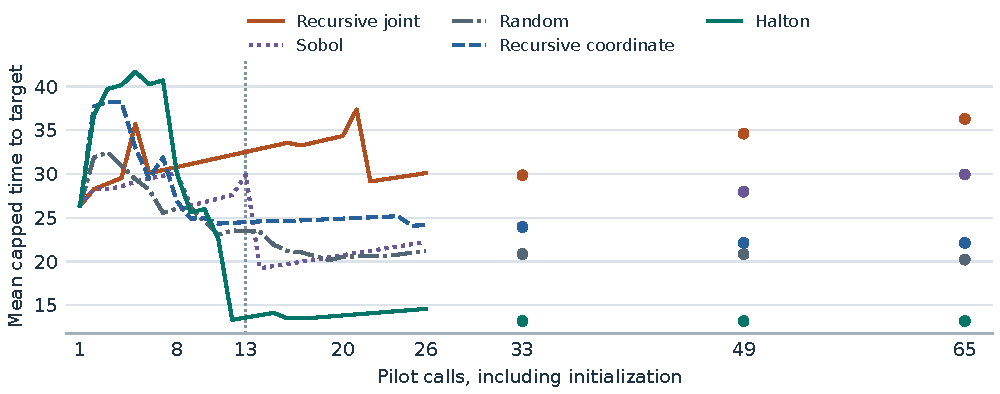
\includegraphics[width=.95\linewidth]{figures/switch_sweep.pdf}\end{center}
\figcaption{2}{Cohort A sensitivity to the pilot length. Smaller capped time is better. Lines connect all integer splits 1--26, and dots show 33, 49 and 65. At $k=65$ the entire budget goes to the pilot. The dotted vertical line marks 13. Full results include both original-sieve curves.}

Among genuine fixed hybrids tested on the historical cases ($1<k<65$), the smallest loss-minimizing $k$ was 33 for Halton, 2 for each joint dyadic order and Sobol, 9 for each coordinate sieve, and 49 for random sampling. If immediate polling was also eligible, its mean of 10 calls won on the historical graphs. Cohort A gives a different ranking. A 33-call Halton pilot and uninterrupted Halton sampling both hit every target by call 28. Local refinement after 33 consequently gets no credit for their first hits.

\newpage
\sect{5}{Should the switch depend on recent progress?}
The learned rule chose the same action in both progress classes for five of seven starters. For Halton it chose to \emph{continue} on a stale prefix. In 11 historical stale cases, stopping at 8 averaged 25.45 capped calls and waiting to 13 averaged 10.00. On the four improving cases the estimates were 40.50 and 40.75, a quarter-call difference favoring an early switch. These small training cells make the distinction fragile. For Sobol the directions reversed: stop on a stale prefix, continue on an improving one.

\tabcaption{3}{Fresh confirmation cohort B. Each hit column counts graph/start cases out of 72. All pilots in this table use Halton. Capped time scores a miss at 66, while Used records the actual calls.}
\begin{center}\small\begin{tabular}{@{}lrrrrr@{}}\toprule
Policy & Mean pilot & Hits @20 & Hits @65 & Capped time & Used\\\midrule
\DecisionRows\bottomrule
\end{tabular}\end{center}

\begin{center}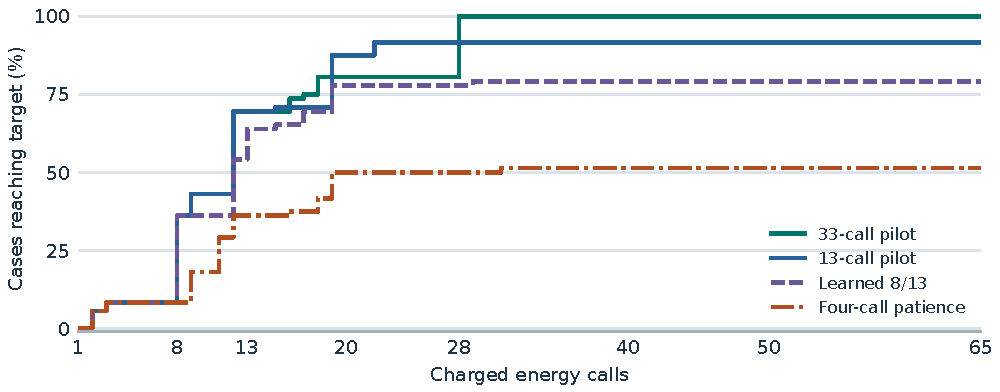
\includegraphics[width=.93\linewidth]{figures/confirmation.pdf}\end{center}
\figcaption{3}{Confirmation first-hit curves. The 33-call pilot and Halton-only curves coincide because every case hits by call 28. The 13-call pilot has more hits at call 20, but finishes with six misses.}

At the 65-call cap, the learned switch reached 57 targets, versus 66 for fixed 13. Its mean capped time was 6.50 calls higher (paired 95\% interval 3.40 to 9.67). Patience reached 37 targets and cost 22.19 additional capped calls (17.22 to 27.17). Fixed 33 gained six final hits over fixed 13 (8.3 percentage points, interval 2.8 to 13.9), while its mean capped-time advantage of 2.44 calls had an interval spanning zero ($-0.13$ to $5.44$ calls saved). Intervals use 10,000 paired bootstrap draws of whole graphs within the six size/density strata. They describe uncertainty within this graph design. The multiple comparisons are descriptive.

\newpage
\sect{6}{Why the starting order matters}
There is a concrete obstruction to using a short joint dyadic prefix on these landscapes. For MaxCut the cost operator $H_C$ commutes with the global bit flip $X^{\otimes n}$, since complementing a cut preserves its size. The mixer obeys
\[
 U_B(\beta+\pi/2)=(-i)^n X^{\otimes n}U_B(\beta),
 \qquad E(\gamma,\beta+\pi/2)=E(\gamma,\beta).
\]
For both Morton-decoded dyadic orders, the first 16 points including the common start form a translated $4\times4$ lattice. Only the top two bits of each coordinate vary. Each $\beta$ offset is a multiple of $\pi/2$, leaving all 16 points in a single $\beta$ equivalence class. At $k=13$ there are only four distinct $(\gamma,\beta\bmod\pi/2)$ pairs. Halton visits 13 such pairs across all four $\beta$ classes on the same grid. This is a property of this encoding and objective. It also gives a reason that several fruitless calls can be a misleading signal about the value of the next, finer points.

\subt{Changing the budget or grid}
On cohort A at $B=33$, the 20\% pilot rounds to seven calls. Halton then hit the target in 35/72 cases, versus 50/72 for immediate pattern search and 72/72 for Halton alone. On the finer $32\times32$ grid with $B=65$, the 13-call Halton pilot hit 18/18 on the six-graph subset, compared with 13/18 for immediate polling. The finer grid sets its own exhaustive reference. These checks show why a fixed percentage needs validation at the intended budget and resolution.

\subt{Choosing a start for the observed geometry}
On the native confirmation grids, every valid key was isolated and the short recursive prefix sampled symmetry-equivalent energies. A 13-call Halton start gave better early coverage here. A 33-call Halton start hit every target in both cohorts before its local phase. The four-call stall and the learned checkpoint lost coverage against fixed 13. The companion's one-block reindexing of the same confirmation energies favored the recursive start at the same 13-call handoff \cite{clusterstudy}. The choice of initializer therefore depends on the order of valid keys. These results measure classical energy queries on noiseless one-layer circuits.

\subt{Reproducibility}
{\footnotesize The companion directory contains the optimizer entry points, graph edge lists, all policy records, fitted rules, paired intervals and figure generation instructions. The original experiment is pinned to repository commit \texttt{0ab4abc}.\par}
\begingroup\footnotesize
\renewcommand{\refname}{\sffamily\small\color{teal}References}
\begin{thebibliography}{9}\setlength{\itemsep}{0pt}\setlength{\parskip}{0pt}
\bibitem{rikula} P. Rikula. \emph{Coarse-to-Fine Dyadic Sampling: An Exact First-Hit Result and an Exploratory QAOA Benchmark}. Zenodo, 2026. \href{https://doi.org/10.5281/zenodo.24382960}{DOI 10.5281/zenodo.24382960}. \href{https://github.com/kummahiih/variational-quantum-algorithms/tree/0ab4abc6ea3a980cd86ac77447979b5e469b54d5/paper}{Archived paper and data}.
\bibitem{farhi} E. Farhi, J. Goldstone and S. Gutmann. A Quantum Approximate Optimization Algorithm. 2014. \href{https://arxiv.org/abs/1411.4028}{arXiv:1411.4028}.
\bibitem{halton} J. H. Halton. On the efficiency of certain quasi-random sequences of points in evaluating multi-dimensional integrals. 1960. \href{https://doi.org/10.1007/BF01386213}{Numerische Mathematik 2, 84--90}.
\bibitem{sobol} I. M. Sobol'. On the distribution of points in a cube and the approximate evaluation of integrals. 1967. \href{https://doi.org/10.1016/0041-5553(67)90144-9}{USSR Comput. Math. Math. Phys. 7, 86--112}.
\bibitem{torczon} V. Torczon. On the convergence of pattern search algorithms. 1997. \href{https://doi.org/10.1137/S1052623493250780}{SIAM J. Optim. 7, 1--25}.
\bibitem{wolniak} M. Wolniak et al. Uncertainty propagation via sample-based deterministic model updating for structural damage identification. 2025. \href{https://doi.org/10.1177/14759217251387535}{Structural Health Monitoring}.
\bibitem{clusterstudy} Variational Quantum Algorithms project. \emph{Clustered versus isolated target keys in QAOA pattern search}. 2026. \href{https://github.com/kummahiih/variational-quantum-algorithms/blob/main/paper/clusters/cluster_assumption.pdf}{Companion matched experiment}.
\end{thebibliography}
\endgroup
{\footnotesize\textbf{Declaration of generative AI assistance.} OpenAI Codex implemented the experiment, ran the simulations, and drafted the analysis and manuscript at the project owner's request. This research draft awaits author review.\par}
\end{document}
